\section{splittable Task}

In the previous chapter we proposed an analytical model to estimate the execution time of a balanced parallel for loop in terms of the grain size. Based on this model, we offered an approach to find the range of grain size to achieve minimum execution time. The parameters of the proposed model are identified through a benchmark and are exposed to the Blaze library to predict the range of grain size for minimum execution time of a problem at run-time. So the proposed method is a combination of compile-time and run-time solution to improve the performance.\\
In this chapter we choose another direction and look into a run-time adaptive solution to control task granularity in order to achieve the minimum execution time. Why? unbalanced work load.

Utilizing splittable tasks is a runtime adaptive method for managing task granularity, to avoid the large overhead of creating and managing too many tasks due to the fine grain parallelism on one hand, and the starvation resulted from creating less tasks than the available parallelism on the other hand.\\ 
Splittable tasks are tasks that could be partitioned into smaller tasks, when sufficient parallelism is available~\cite{prell2016embracing}. 

~\cite{robison2008optimization}

Prell intensively studies using the splittable tasks for runtime adaptivity in ~\cite{prell2016embracing}. They start by offering steal-half strategy for work stealing in order to steal half of the tasks from a worker's queue at each steal attempt instead of just one task. This could help to avoid creating too much work stealing overhead. But depending on the application, steal-one or steal-half might be the preferable method for work stealing. They propose an adaptive method to decide on whether to use steal-one or steal-half strategy at runtime, based on the current selected strategy and the ratio of the number of executed tasks($M$) within the last $N$ steals, where $N$ is considered the evaluation interval~\cite{prell2016embracing}.\\ 
Next, basing on lazy task scheduling~\cite{tzannes2014lazy}, they suggest to instead of creating at the tasks and decide on how to the workers should steal them, we can create one task and let it split if needed. This way you wouldn't have to deal with the overhead of scheduling tasks along with the overhead of stealing the tasks.\\
At each split, a portion of the task would be added to the current worker's deque as a splittble task to be stolen by free workers, while the rest of the task would be executed by the current worker.    
They propose two splitting strategies namely, and adaptive. 


Our work here is based on Prell~\cite{prell2016embracing}'s definition of splittable tasks and their split strategies. We have implemented an executor within HPX which would create splittable tasks to execute the work, and we improved upon their work in following ways:

\begin{itemize}
\item At each split, instead of allowing the created splittable task to be stolen by free workers, we turn work stealing off, identify the idle workers and explicitly assign the work to one of them. This way we avoid the work stealing overhead originated from unsuccessful steal attempts. 
\item We suggest to utilize our proposed method for identifying the range of grain size for minimum execution time, and use the lower-bound of the range as a cutoff value to stop splitting in order to avoid creating too fine tasks.   
\item We used Apex, an Autonomic Performance Environment for Exascale~\cite{huck2015autonomic}, as a profiling tool to study how tasks are being scheduled.
\end{itemize}




\subsection{Implementation}
For a parallel for-loop with the range of $[a,b)$, one splittable task containing all the iterations from $a$ to $(b-1)$ would be created. Depending on the splitting strategy when a certain condition is met this task would be split into two tasks, $task_1$ containing iterations in the range of $[a,c)$ and $task_2$ would contain iterations from $[c,b)$, where $c$ is the split point. $task_1$ would be executed by the current worker while $task_2$, which is also a splittable task, would be scheduled to run on another core. This allows the runtime to adaptively decide whether to split the current task into smaller tasks or just run it.     

 
\subsection{Splitting Strategies}
The splittable task could be split either based on total number of cores available, or number of idle cores at the time of split. 

\subsubsection{Splitting based on total number of cores}

\subsubsection{Splitting based on number of idle cores}

\subsection{Results}

\subsubsection{For-loop Benchmark}

\begin{figure}[H]
	\centering
	\subfloat[]
	{\centering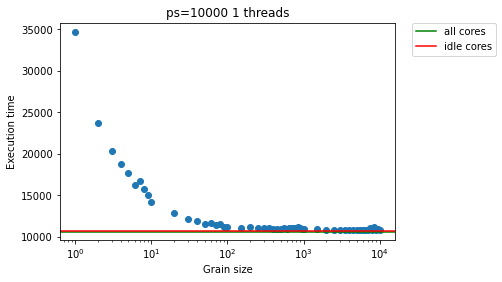
\includegraphics[scale=.35]{images/hpx_for_loop/splittable/all_idle_cores/marvin_10000_1.png}	
		\label{fig66:a}}
	\subfloat[]
	{\centering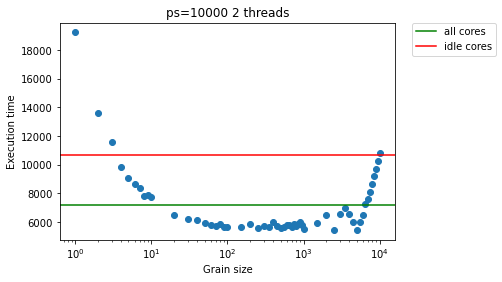
\includegraphics[scale=.35]{images/hpx_for_loop/splittable/all_idle_cores/marvin_10000_2.png}	
		\label{fig66:b}}\hfill
	\subfloat[]
	{\centering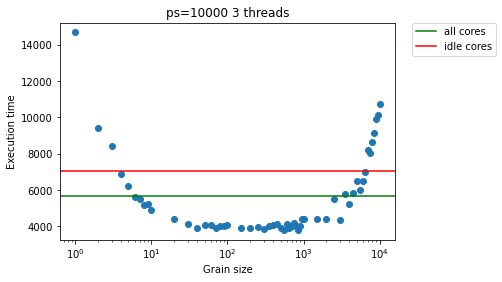
\includegraphics[scale=.35]{images/hpx_for_loop/splittable/all_idle_cores/marvin_10000_3.png}	
		\label{fig66:c}}
	\subfloat[]
	{\centering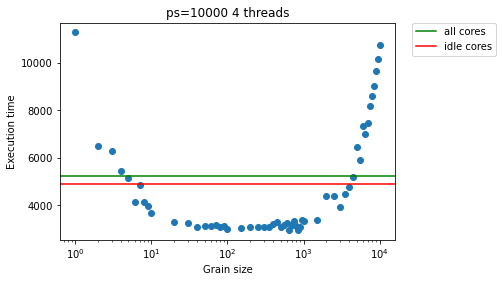
\includegraphics[scale=.35]{images/hpx_for_loop/splittable/all_idle_cores/marvin_10000_4.png}	
		\label{fig66:d}}\hfill
	\subfloat[]
	{\centering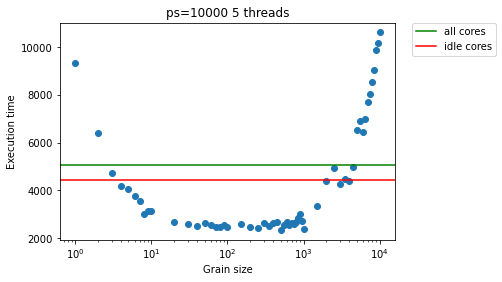
\includegraphics[scale=.35]{images/hpx_for_loop/splittable/all_idle_cores/marvin_10000_5.png}	
		\label{fig66:e}}
	\subfloat[]
	{\centering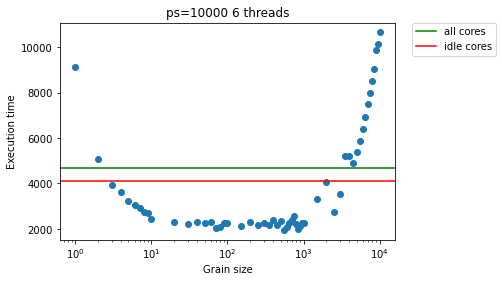
\includegraphics[scale=.35]{images/hpx_for_loop/splittable/all_idle_cores/marvin_10000_6.png}	
		\label{fig66:f}}\hfill
	\subfloat[]
	{\centering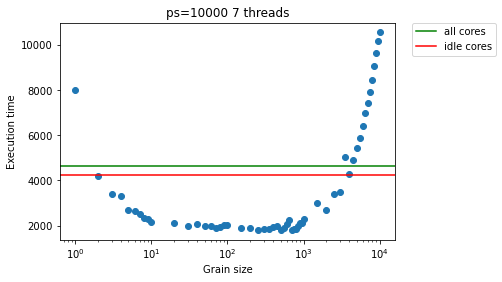
\includegraphics[scale=.35]{images/hpx_for_loop/splittable/all_idle_cores/marvin_10000_7.png}	
		\label{fig66:g}}
	\subfloat[]
	{\centering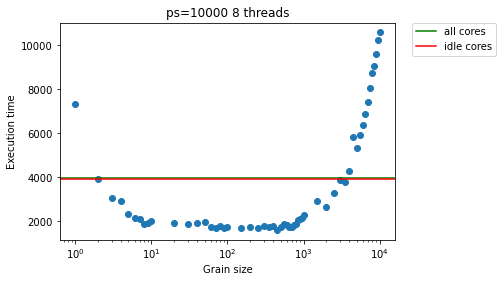
\includegraphics[scale=.35]{images/hpx_for_loop/splittable/all_idle_cores/marvin_10000_8.png}	
		\label{fig66:h}}\hfill
	\caption{The results of running the hpx for loop using splittable tasks with all-cores and idle-cores split types compared with different grain sizes, for $problem\_size=10000$, for (a) 1 core, (b) 2 cores, (c) 3 cores, (d) 4 cores, (e) 5 cores, (f) 6 cores, (g) 7 cores, (h) 8 cores. The unit for execution time is microseconds.}
	\label{fig66}	
\end{figure}

\subsubsection{Blazemark}

\subsubsection{Apex}